% Created 2022-10-16 Sun 05:58
% Intended LaTeX compiler: xelatex
\documentclass[a4paper,11pt]{article}
\usepackage{graphicx}
\usepackage{longtable}
\usepackage{wrapfig}
\usepackage{rotating}
\usepackage[normalem]{ulem}
\usepackage{amsmath}
\usepackage{amssymb}
\usepackage{capt-of}
\usepackage{hyperref}
\usepackage{kotex}
\RequirePackage[math-style=TeX,bold-style=TeX]{unicode-math}
\setmainfont{Libertinus Serif}
\setsansfont{Libertinus Sans}[Scale=MatchUppercase]
\setmonofont{Inconsolata}[Scale=MatchLowercase]
\setmathfont{Libertinus Math}[Scale=MatchUppercase] % Before set*hangulfont
\setmainhangulfont{Noto Serif CJK KR}[Scale=.885]
\setsanshangulfont[BoldFont={* Bold}]{KoPubWorldDotum_Pro}[Scale=.885]
\setmonohangulfont{D2Coding}[Scale=MatchLowercase]
\author{이재호}
\date{10/16/22}
\title{모나드 발명하기}
\hypersetup{
 pdfauthor={이재호},
 pdftitle={모나드 발명하기},
 pdfkeywords={},
 pdfsubject={},
 pdfcreator={Emacs 29.0.50 (Org mode 9.5.5)}, 
 pdflang={English}}
\begin{document}

\maketitle
\tableofcontents

\begin{center}

\includegraphics[width=.9\linewidth]{./monad.jpeg}
\end{center}

\section{왜?}
\label{sec:org0ae2cd8}
\subsection{그래서 모나드가 뭔데?}
\label{sec:org3fb5b61}
\begin{quote}
모나드는 자기 함자 범주에서의 모노이드인데, 뭐가 문제야?
A monad is a monoid in the category of endofunctors, what's the problem?
\end{quote}
\url{http://james-iry.blogspot.com/2009/05/brief-incomplete-and-mostly-wrong.html}


\subsection{지금까지 문제 없었는데?}
\label{sec:org0da5715}
\begin{center}
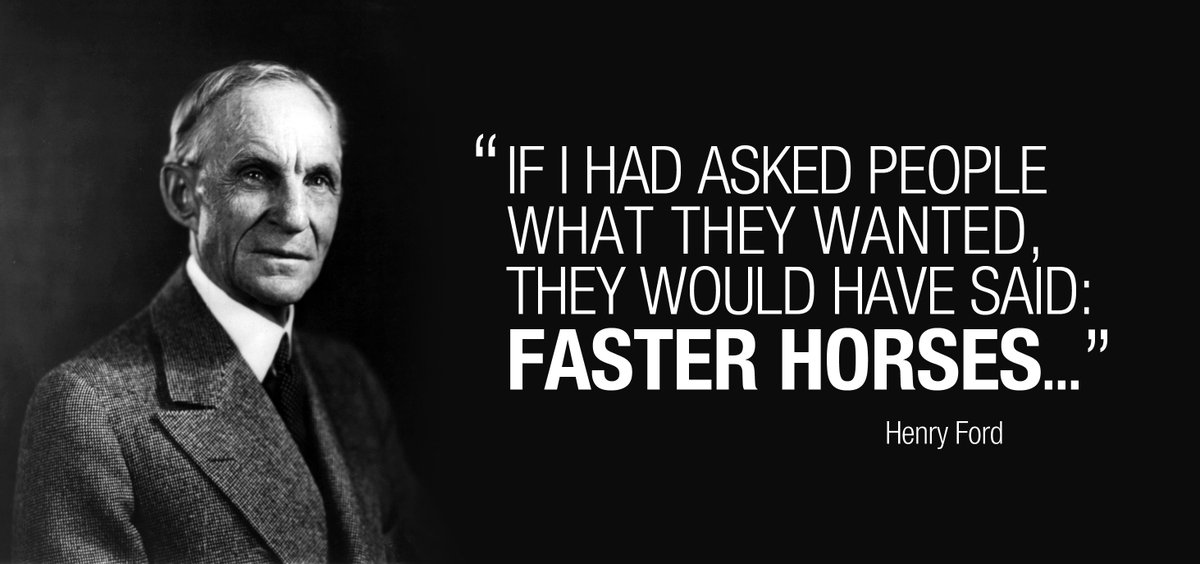
\includegraphics[width=.9\linewidth]{./faster-horse.jpg}
\end{center}
\begin{itemize}
\item 과장 조금 (많이) 보태서, 그냥 튜링 머신으로도 문제 없다!
\end{itemize}

\subsection{구조적 프로그래밍}
\label{sec:org295b28c}
\begin{center}
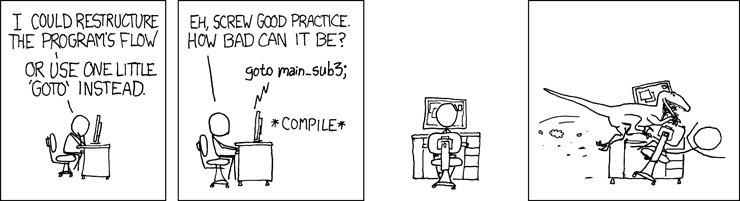
\includegraphics[width=.9\linewidth]{./goto.png}
\end{center}

\begin{quote}
\ldots{} 우리의 지력은 정적인 관계를 파악하는데에 적합하지, 시간에 따라 과정이 어떻게 흘러가는지 시각화하는 것에는 다소 약하다. \ldots{}
\begin{itemize}
\item 에츠허르 W. 다익스트라, "Go To문의 해로움에 관하여"
\end{itemize}
\ldots{} our intellectual powers are rather geared to master static relations and that our powers to visualize processes evolving in time are relatively poorly developed. \ldots{}
\begin{itemize}
\item Edsger W. Dijkstra in "Go To Statement Considered Harmful"
\end{itemize}
\end{quote}

\begin{itemize}
\item 한 단계 위에서 이해하기
\begin{itemize}
\item 기계의 조종이라는 개념이 아니라, 논리적인 구조를 기반으로 사고
\end{itemize}
\item 사실 제약은 '기능'
\begin{itemize}
\item 프로그래밍 언어는 우리에게서 자유도를 빼앗아가며 발전
\item Lisp (1950): 조건문, 일급 시민인 함수 (+재귀), 쓰레기 처리
\end{itemize}
\end{itemize}

\subsection{우리(프로그래머)를 편하게 해주는 것들}
\label{sec:org97cd77e}
\begin{itemize}
\item 문법 설탕도 우리의 삶을 윤택하게 해주지만, 깊이가 매우 얕음
\begin{itemize}
\item 쉽지만 상당수는 작은 이득만을 가져다 줌
\end{itemize}
\item 반면 더 깊은 수준에서 우리를 도와주는 도구들도 있음: 타입 이론, 쓰레기 처리기, 구조적 동시성, \ldots{}
\begin{itemize}
\item 하지만 프로그래머에게 일정 수준 이상의 공부와 규율을 요구함
\item 매우 큰 보상을 줌
\end{itemize}
\end{itemize}

\subsection{모나드}
\label{sec:orgced337a}
"계산이란 무엇인가?"
\begin{itemize}
\item 사실은 순수한 프로그래밍 언어인 하스켈의 입출력을 위해서 프로그래밍 세계에 실제로 도입됨
\item 프로그램 실행의 관점에서 다른 방향의 고수준 생각을 열어줌
\end{itemize}

\section{발명하기}
\label{sec:org50a407f}
일단은 실용적인 방향으로\ldots{}

\subsection{백만불 아끼기}
\label{sec:orgf03e1da}
The Billion Dolloar Mistake:
\url{https://www.infoq.com/presentations/Null-References-The-Billion-Dollar-Mistake-Tony-Hoare/}

\subsubsection{문제 상황}
\label{sec:orgf1ff9ef}
사용자별로 시간표 하나씩 있고, 시간표를 확인하여 수업들을 볼 수 있는 구조:
\begin{verbatim}
class User:
    def __init__(self, name, timetable_id):
        self.name = name
        self.timetable_id = timetable_id

class Timetable:
    def __init__(self, name, classes):
        self.name = name
        self.classes = classes

USERS = {
    "c9f4ad09-3a57-449e-9303-39fc618ba4a8": User(
        "jay",
        "bd96da54-5202-4e74-947d-a68c6e50c941"
    ),
}

TIMETABLES = {
    "bd96da54-5202-4e74-947d-a68c6e50c941": Timetable(
        "2022 Fall",
        ["class 1", "class 2"]
    ),
}
\end{verbatim}

사용자의 ID를 통해 수업들을 확인할 수 있도록 돕는 함수들:
\begin{verbatim}
def get_user(user_id):
    return USERS[user_id]

def get_timetable(user):
    return TIMETABLES[user.timetable_id]

def get_classes(timetable):
    return timetable.classes

uid = "c9f4ad09-3a57-449e-9303-39fc618ba4a8"
print(f"{get_classes(get_timetable(get_user(uid))) = }")
\end{verbatim}

만약 없는 사용자의 ID를 넣어준다면?
\begin{verbatim}
uid2 = "63a212d5-11e9-4bee-80de-c1d2c12f0478"
try:
    print(get_classes(get_timetable(get_user(uid2))))
except:
    import traceback
    traceback.print_exc()
\end{verbatim}

\subsubsection{해결법}
\label{sec:orga91bd9d}
\begin{itemize}
\item 예외 사용하기
\end{itemize}
파이썬을 포함한 현대적인 프로그래밍 언어들에 모두 들어간 예외를 사용해 처리 가능!
\begin{verbatim}
try:
    classes = get_classes(get_timetable(get_user(uid2)))
except:
    classes = None
print(classes)
\end{verbatim}

\begin{itemize}
\item 타입 수준에서 해결: \texttt{Optional} 사용하기 (\texttt{T | None = Optional[T]})
\begin{itemize}
\item 안전한 함수들을 만들자
\end{itemize}
\end{itemize}
\begin{verbatim}
def get_user_safe(user_id: str) -> User | None:
    return USERS.get(user_id)

def get_timetable_safe(user: User) -> list[str] | None:
    return TIMETABLES.get(user.timetable_id)
\end{verbatim}

\begin{verbatim}
try:
    # 바로 이렇게는 사용하지 못하지만...
    print(get_classes(get_timetable_safe(get_user_safe(uid2))))
except:
    import traceback
    traceback.print_exc()
\end{verbatim}

복잡하긴 하지만 이렇게 사용 가능:
\begin{verbatim}
def safe_call(user_id):
    user = get_user_safe(user_id)
    if user is None:
        return None
    timetable = get_timetable_safe(user)
    if timetable is None:
        return None
    return get_classes(timetable)


print(f"{safe_call(uid) = }")
print(f"{safe_call(uid2) = }")
\end{verbatim}

\subsubsection{편하게 쓸 수 있게 감싸 보자}
\label{sec:org621a595}
\begin{verbatim}
from typing import TypeVar, Callable, Generic

T = TypeVar("T")
U = TypeVar("U")

class Packet(Generic[T]):
    def __init__(self, payload: T | None):
        self.payload = payload

    def if_exists(self, f: Callable[[T], U | None]) -> "Packet[U]":
        if self.payload is None:
            return self
        return Packet(f(self.payload))
\end{verbatim}

\begin{verbatim}
def get_classes_from_user(user_id):
    return Packet(get_user_safe(user_id)) \
        .if_exists(get_timetable_safe) \
        .if_exists(get_classes)


print(get_classes_from_user(uid).payload)
print(get_classes_from_user(uid2).payload)
\end{verbatim}

\subsubsection{\texttt{get\_classes\_from\_user(...) -> Packet[...]}?!}
\label{sec:org40b53ed}
\texttt{Packet} 을 돌려주는 다른 함수와는 \texttt{if\_exists} 로 감싸면 계속 \texttt{Packet} 으로 감싸지는데\ldots{}
\begin{verbatim}
class ClassCounterService:
    def __init__(self):
        return

    def count_classes(self, classes: list[str]) -> Packet[int]:
        return Packet(len(classes))

SHARED_CLASS_COUNTER = ClassCounterService()

def get_class_count(classes: list[str]) -> Packet[int]:
    return SHARED_CLASS_COUNTER.count_classes(classes)

class_cnt = get_classes_from_user(uid).if_exists(get_class_count)
print(f"{type(class_cnt) = }")
print(f"{type(class_cnt.payload) = }")
print(f"{type(class_cnt.payload.payload) = }")
print(f"{class_cnt.payload.payload = }")
\end{verbatim}

\begin{center}

\includegraphics[width=.9\linewidth]{./matroshka.jpg}
\end{center}

\subsubsection{까서 합체하자!}
\label{sec:org08c551e}
\begin{verbatim}
class Packet(Generic[T]):
  def __init__(self, payload: T | None):
      self.payload = payload

  def if_exists(self, f: Callable[[T], U | None]) -> "Packet[U]":
      if self.payload is None:
          return self
      return Packet(f(self.payload))

  def if_exists_coalesce(self, f: Callable[[T], "Packet[U]"]) -> "Packet[U]":
      if self.payload is None:
          return self
      return f(self.payload)
\end{verbatim}

\begin{verbatim}
def get_classes_from_user(user_id):
    return Packet(get_user_safe(user_id)) \
        .if_exists(get_timetable_safe) \
        .if_exists(get_classes)

class ClassCounterService:
    def __init__(self):
        return

    def count_classes(self, classes: list[str]) -> Packet[int]:
        return Packet(len(classes))

SHARED_CLASS_COUNTER = ClassCounterService()

def get_class_count(classes: list[str]) -> Packet[int]:
    return SHARED_CLASS_COUNTER.count_classes(classes)

class_cnt = get_classes_from_user(uid).if_exists_coalesce(get_class_count)
print(f"{type(class_cnt) = }")
print(f"{type(class_cnt.payload) = }")
print(f"{class_cnt.payload = }")
\end{verbatim}

\subsection{아마도 모나드 (Maybe Monad)}
\label{sec:org3a429be}
그냥 (Just) 값이 들어있거나 없거나 (Nothing).

위의 \texttt{Packet} 이 아마도 모나드!
\begin{itemize}
\item \texttt{\_\_init\_\_} 으로 \texttt{T} 를 감쌀 수 있고("return"), \texttt{\_if\_exists\_coalesce} 로 다른 아마도 모나드 (\texttt{Packet})를 돌려주는 함수와 이을 수 있다("bind").
\end{itemize}

\subsubsection{잠깐 길을 벗어나서: 문법 설탕}
\label{sec:org9c6ce68}
문법 설탕을 통해서 모나드를 자연스럽게 사용할 수 있다.

대입도 문법 설탕!
\begin{verbatim}
a = 1
b = a * 2
c = 3
print(a + b + c)
\end{verbatim}

\begin{verbatim}
(lambda a:
 (lambda b:
  (lambda c:
   print(a + b + c)
   )(3)
  )(a * 2)
 )(1)
\end{verbatim}

즉, \texttt{\textasciitilde{}x = y \textbackslash{}n ... \textasciitilde{}} 은 사실 함수 적용의 문법 설탕

\textbf{이하는 유사-파이썬 코드입니다.}
\begin{enumerate}
\item 1단계 문법 설탕
\label{sec:org0b0f6d1}
중위 연산자 정의가 가능한 언어라면 다음과 같이 "="을 만들어낼 수 있다.
\begin{verbatim}
1 >>= (lambda a:
  a * 2 >>= (lambda b:
    3 >>= (lambda c:
      print(a + b + c)
    )
  )
)
\end{verbatim}

\item 2단계 문법 설탕
\label{sec:org2c00f69}
";"을 갈아끼울 수 있는 언어라면 다음과 같이 "="을 만들어낼 수 있다.
\begin{verbatim}
a = 1
b = a * 2
c = 3
print(a + b + c)
\end{verbatim}

\item 아마도 모나드의 의미로 "="을 갈아끼우자
\label{sec:org99b5522}
"C1; C2"은 "C1"를 한 후 "C2"를 하라는 의미인데, 이 의미를 갈아끼우는 것!

\begin{enumerate}
\item Haskell
\label{sec:orge447b01}
\begin{verbatim}
do a <- Just 1
   b <- Just (a * 2)
   c <- Just 3
   return (a + b + c)
\end{verbatim}

\item OCaml
\label{sec:orgbe4def9}
\begin{verbatim}
let* a = Some 1 in
let* b = Some (a * 2) in
let* c = Some 3 in
return (a + b + c)
\end{verbatim}

일반적인 대입과 비교하면 의미심장하다:
\begin{verbatim}
let a = 1 in
let b = a * 2 in
let c = 3 in
a + b + c
\end{verbatim}
\end{enumerate}
\end{enumerate}

\section{모나드}
\label{sec:org75c98e0}
\begin{itemize}
\item 모기(Moggi): \(f: A \to B\) 처럼 생긴 "함수"는 사실 수학적인 함수가 아니라, \(f: A \to M\,B\) 인 수학적인 함수로 표현 가능
\begin{itemize}
\item \(A\) 라는 타입의 값과 \(M\ A\) 라는 타입의 "계산"을 분리
\end{itemize}
\item 예시
\begin{enumerate}
\item 부분 정의: \(M\,A = A_\bot\)
\item 비결정성: \(M\,A = \wp(A)\)
\item 부작용: \(M\,A = S \to A \times S\)
\item 예외: \(M\,A = A + E\)
\end{enumerate}
\end{itemize}

\subsection{게임의 규칙}
\label{sec:orgd8ac2eb}
\begin{itemize}
\item \texttt{bind: 'a t -> ('a -> 'b t) -> 'b t} 와 \texttt{return: 'a -> 'a t} 의 구현
\begin{itemize}
\item 언어별로 타입을 조금씩 다르게 표현: \texttt{'a t} OCaml, \texttt{t<a>} TypeScript/C++/Swift/ReScript/\ldots{}, \texttt{t[a]} Python, \texttt{t a} Haskell/Elm/\ldots{}
\end{itemize}
\item 모나드 법칙
\begin{enumerate}
\item \texttt{bind(return(o), f) == f(a)}
\begin{itemize}
\item Python 등 OOP 언어에서는 \texttt{return(o).bind(f)} 와 같이 읽으면 된다
\end{itemize}
\item \texttt{bind(m, return) == m}
\begin{itemize}
\item 마찬가지로 \texttt{m.bind(return)}
\end{itemize}
\item \texttt{bind(bind(m, f), g) = bind(m, lambda a: bind(f(a), g))}
\begin{itemize}
\item \texttt{m.bind(f).bind(g) = m.bind(lambda a: f(a).bind(g))}
\item 이게 무슨 의미인지는 아래 \hyperref[org9729d4a]{비결정성}에서 확인
\end{itemize}
\end{enumerate}
\end{itemize}

\subsection{아마도 (Maybe)}
\label{sec:orgba3c8b1}
파이썬은 타입이 명시적으로 드러나지 않으므로 정적 타입 언어로 다시 정리하자면:
\begin{verbatim}
(* type 'a option = None | Some of 'a (* Built-in *) *)
let return (x : 'a) : 'a option = Some x
let bind (o : 'a option) (f : 'a -> 'b option) : 'b option = match o with
| None -> None
| Some x -> f x
\end{verbatim}

\subsection{리스트}
\label{sec:orgf243b2f}
\begin{verbatim}
(* type 'a list = [] | (::) of 'a * 'a list (* Built-in *) *)
let return (x : 'a) : 'a list = [ x ]
let bind (o : 'a list) (f : 'a -> 'b list) : 'b list = List.concat_map f o
\end{verbatim}

\begin{verbatim}
class ListMonad(Generic[T]):
  def __init__(self, lst: list[T]):
      self.lst = lst

  def bind(self, f: Callable[[T], list[U]]) -> list[U]:
      return ListMonad([y for x in self.lst for y in f(x).lst])  # ?!
\end{verbatim}

\begin{verbatim}
nums = ListMonad([1, 2, 3])
print(nums.bind(lambda x: ListMonad([x, x * 2, x * 3]) if x % 2 == 0 else ListMonad([])).lst)
print(f"{[a for x in [1, 2, 3] if x % 2 == 0 for a in [x, x * 2, x * 3]] = }")
\end{verbatim}

한 겹의 괄호에 리스트를 주는 for-식이 들어가는 것은 사실상 모나드를 사용한 코드이다!

하지만 리스트 표현식의 한계는 다음 OCaml 코드의 가독성에서 확인할 수 있다:
\begin{verbatim}
let ( let* ) = bind

let result =
  let* x = [1; 2; 3] in
  if x mod 2 = 0 then
    [x; x * 2; x * 3]
  else
    []
\end{verbatim}

\subsection{비결정성}
\label{sec:org75a5699}
\label{org9729d4a}
비결정적인 프로그램의 "의미(semantics)"를 리스트로 표현 가능
\begin{verbatim}
# Inspired by https://stackoverflow.com/a/20644753
import enum

class CoinType(enum.Enum):
    FAIR = enum.auto()
    BIASED = enum.auto()

class Coin(enum.Enum):
    HEAD = enum.auto()
    TAIL = enum.auto()

def toss(coin):
    match coin:
        case CoinType.FAIR:
            return ListMonad(list(Coin))
        case CoinType.BIASED:
            return ListMonad([Coin.HEAD, Coin.HEAD])

def pick():
    return ListMonad(list(CoinType))

print(pick().bind(toss).bind(lambda result: ListMonad([result] if result == Coin.HEAD else [])).lst)
print(pick().bind(lambda coin:
    toss(coin).bind(lambda result:
        # `coin` is now in scope here!
        # See the monad law 3 in action
        ListMonad([coin] if result == Coin.HEAD else []))
    ).lst
)
\end{verbatim}

이거 그냥 map으로는 안되나? -> [] 때문에 안 됨

\section{마음가짐}
\label{sec:org147dacd}
\begin{itemize}
\item 명령형 프로그래밍에서의 함수 \(f: A \to B\) 는 수학적으로는 적절한 모나드 \$M\$에 대한 \(f: A \to M\,B\) 으로 항상 나타낼 수 있다.
\item 리스트 연산을 할 때, 중첩된 map과 flatmap, filter를 난발하기 전에 한 발짝 물러서서 내가 지금 무엇을 하고 있는지 타입 수준에서 생각해보자.
\item None이 될 수 있는 타입(옵션, 옵셔널, 널러블, \ldots{})에 대한 연산, 리스트의 연산, 프로미스의 연산, 예외를 뱉는 연산은 모두 동일한 방식의 변환을 사용한다.
\item Python의 리스트 표현식, Swift의 flatMap과 Optional에 관한 \texttt{??}, \texttt{?.}, \texttt{if let} 등의 문법 설탕 등등 특정 모나드에 대한 조준 사격이 사실은 일반화 가능하다.
\item 모나드는 "세미콜론"의 일반화이다.
\item 모나드는 자기 함자 범주에서의 모노이드인데, 뭐가 문제야?
\end{itemize}

\subsection{참고}
\label{sec:org8c0e8fe}
\url{https://github.com/Zeta611/L/commit/68cd96611a4ac719a21ee4dcb09d9c16def7edbf}
\end{document}